\documentclass{report}
\usepackage[utf8]{inputenc}     % for éô
\usepackage[english]{babel}     % for proper word breaking at line ends
\usepackage[a4paper, left=1.5in, right=1.5in, top=1.5in, bottom=1.5in]{geometry}
% for page size and margin settings
\usepackage{graphicx}           % for ?
\usepackage{amsmath,amssymb}    % for better equations
\usepackage{amsthm}             % for better theorem styles
\usepackage{mathtools}          % for greek math symbol formatting
\usepackage{varwidth}
\usepackage{enumitem}           % for control of 'enumerate' numbering
\usepackage{listings}           % for control of 'itemize' spacing
\usepackage{todonotes}          % for clear TODO notes
\usepackage[hidelinks]{hyperref}           % page numbers and '\ref's become clickable
\usepackage{pgfplots}
\usepackage{caption}
\usepackage{parskip}
\usepackage{makecell}
\usepackage{tabularx}


% \pgfplotsset{width=10cm,compat=1.9}


% Listing style

%% Package for colors.
\usepackage{xcolor}
%% Useful colors
\definecolor{blue}{RGB}{0,0,255}
\definecolor{codegreen}{rgb}{0,0.6,0}
\definecolor{codegray}{rgb}{0.5,0.5,0.5}
\definecolor{codepurple}{rgb}{0.58,0,0.82}
\definecolor{backcolour}{rgb}{1,0.973,0.906}
\definecolor{mygray}{gray}{0.96}

%% Code listing style named "mystyle"
\lstdefinestyle{mystyle}{
    backgroundcolor=\color{mygray},
%commentstyle=\color{codegreen},
%keywordstyle=\color{magenta},
%numberstyle=\tiny\color{codegray},
    stringstyle=\color{codepurple},
    basicstyle=\footnotesize,
    breakatwhitespace=false,
    breaklines=true,
    captionpos=b,
    keepspaces=true,
%   numbers=left,                    
    numbersep=5pt,
    showspaces=false,
    showstringspaces=false,
    showtabs=false,
    tabsize=2
}
% "mystyle" code listing set
\lstset{style=mystyle}


%%%%%%%%%%%%%%%%%%%%%%%%%%%%%%%%
%% SET TITLE PAGE VALUES HERE %%
%%%%%%%%%%%%%%%%%%%%%%%%%%%%%%%%
%             ||               %
%             ||               %
%             \/               %

\newcommand{\thesistitle}{Integrating secure authenticated video calling into PubHubs}
\newcommand{\thesissubtitle}{A design and the need for authenticated video calling}
\newcommand\thesisauthorfirst{Julian van der Horst \\ s1015357}
\newcommand\thesisauthorsecond{}
\newcommand\thesissupervisorfirst{Bart Jacobs}
\newcommand\thesissupervisorsecond{Omar Javed}
\newcommand\thesissecondreaderfirst{TBA}
\newcommand\thesissecondreadersecond{Bram Westerbaan}
\newcommand\thesisdate{Febrauri 2024}


%% FOR PDF METADATA
\title{\thesistitle}
\author{\thesisauthorfirst\space\thesisauthorsecond}
\date{\thesisdate}

%%%%%%%%%%%%%%%%%%%%%%%

\begin{document}
\begin{titlepage}
\thispagestyle{empty}
\newcommand{\HRule}{\rule{\linewidth}{0.5mm}}
\center
\textsc{\Large Radboud University Nijmegen}\\[.7cm]

\includegraphics[width=25mm]{img/in_dei_nomine_feliciter}\\[.5cm]
\textsc{Faculty of Science}\\[0.5cm]

\HRule \\[0.4cm]
{ \huge \bfseries \thesistitle}\\[0.1cm]
\textsc{\thesissubtitle}\\
\HRule \\[.5cm]
\textsc{\large Thesis M.Sc. Computing Science}\\[.5cm]

\begin{minipage}{0.4\textwidth}
    \begin{flushleft}
        \large
        \emph{Author:}\\
        \thesisauthorfirst\space \textsc{\thesisauthorsecond}
    \end{flushleft}
\end{minipage}
~
\begin{minipage}{0.4\textwidth}
    \begin{flushright}
        \large
        \emph{Supervisor:} \\
        \thesissupervisorfirst  \\[1em]
        \emph{Daily supervisor:} \\
        \thesissupervisorsecond \\[1em]
        \emph{Second reader:} \\
        \thesissecondreaderfirst\\
        % \thesissecondreadersecond
    \end{flushright}
\end{minipage}\\[4cm]
\vfill
%{\large \thesisdate}\\
{\large \today}
\end{titlepage}

\tableofcontents

\newpage
\section*{Abstract}


\chapter{Introduction}
PubHubs is a platform which is currently still looking for a suitable use case. Although there are many privacy enhancing features present in PubHubs, many clients will not use it since it lacks features which are required for their use case. We believe that having the ability to video call within PubHubs can be a very useful feature, which for some clients is a necessity.
This way, the privacy-friendly PubHubs can be used for numerous applications, like online consultations, online
classes, or just to have a chat with friends. However, currently there are no organizations which are using PubHubs for this. So it is hard to say what the exact requirements are
for video calling in PubHubs. We will make some requirements in terms of privacy, security, and usability which we
will be in line with the current PubHubs principles. We will then design a video conferencing solution and implement
this design into a prototype. This prototype will be evaluated on the requirements we have set.

\todo{Mention some requirements here}

\chapter{Background}
We first asses the current state of PubHubs as well as the different frameworks and technologies that we will use in
our design. This is needed to fully understand the requirements and design of the video conferencing solution. We
will also discuss what precisely we mean with video conferencing and what the different options are for video
conferencing.

\section{PubHubs}
PubHubs, short for Public Hubs, is an alternative community platform that puts public values first
\cite{jacobs_pubhubs_2023}. Unlike mainstream social media platforms like Instagram or Twitter that focus on
individual broadcasting, PubHubs emulates offline social dynamics by centering interactions within smaller,
community-based hubs. The reasoning
behind that is that this behavior closely resembles offline human interaction, where humans have small groups of
friends and collaborators with whom they interact. Social media now is very unnatural, where if people engage with a
platform, their posts are broadcasted into the whole world and are for everyone to see.

“PubHubs is organized as a network of independent hubs, with a shared single-sign-on. Conversations take place in
local hubs (and not globally) and the associated (conversation) data is managed decentrally, within each hub”~
\cite{jacobs_pubhubs_2023}. The main idea of PubHubs is to allow pseudonymity while maintaining both accountability
and the ability to verify certain attributes of the user. Privacy is one of the core values of PubHubs, which can be
seen in how it handles identity management.

PubHubs consists of a central server(PubHubs central or \textit{PHC}), the Transcryptor (\textit{TS}) and multiple
hubs.
When a user registers, they register at PubHubs central using Yivi (formerly IRMA)\cite{alpar_irma_nodate} by disclosing
certain attributes. When the attributes are verified the user is assigned a global identity by \textit{PHC}.
This global identity (pseudonym) is an Elgamal encryption of the user identity, which no single entity within PubHubs
can decrypt, but if the \textit{PHC} and the \textit{TS} work together they can. In each hub, the user will have a
local identity, which is derived from the global pseudonym. This local identity is created by multiplying the
global pseudonym with a hub specific 'psuedonymization' factor, which is only known by the \textit{TS}. This is set
up in such a way that \textit{PHC} does not learn to which hub the user is going, while \textit{TS} does not learn
who is visiting the hub. This way the user can be anonymous within the hub, and even across hubs, but whenever the
\textit{PHC} and the \textit{TS} work together they can identify the user, for instance when the user is misbehaving.

In PubHubs all communication is done via Matrix. Matrix is an open-source network for secure, decentralized
communication \cite{noauthor_matrixorg_nodate}, which will be explained in \autoref{sec:matrix}. PubHubs can be considered a
layer on top of Matrix, which handles the identity management and adds some extra features like the ability to have
secured rooms.

Secured rooms are rooms which a user can only enter if an attribute is disclosed. For example, a hub can require
that a user has a certain age before they can enter a room. The hub can request these attributes using Yivi. The hub
can then cryptographically verify that the user has the attribute without knowing the actual
value of the attribute. This way, the user can prove that they have the attribute without disclosing the actual
value of the attribute. Staying with the example of age, the hub can verify that the user is over 18 without knowing
the actual age of the user. This is a very powerful feature of PubHubs, which can be used for many different use cases.

In PubHubs the hubs are run by different organizations which typically have a public function, such as
local governments, schools, libraries or hospitals.
These hubs can have different rules or have different features.
To allow this, PubHubs has a strong divide between PubHubs central and the different hubs.
This division is even made in the client, where there is a distinction of the global client and the hub client.

The global client enables a user to go from hub to hub and log in, it is
the interface that you see when you visit the PubHubs website.
Once you enter a hub, the global client loads the hub client in an Iframe. The hub client
is the client that the hub itself deploys. Here, the hubs have full control
over the client. They can control the layout, the features, and the look and feel of the client.

Even in the code base there is a clear distinction between the global client and the hub client.
Although there is a way to communicate between the global client and the hub client, this
is only used to let the hub client know certain settings which are set in the global client.
For example, whether the user prefers a light or dark theme.


\section{Video conferencing}
Video conferencing systems have been around since the 60s and 70s, when NASA used it to communicate with astronauts
on space flights. It has made its appearance in many science fiction works, where it seems like a far-off future.
However, in the last decade, video conferencing has become a standard tool for many businesses and individuals.
Popularity increased dramatically during the COVID-19 pandemic, there was a big need for remote work. Immediately,
services like Zoom \cite{noauthor_one_nodate} and Microsoft Teams  \cite{noauthor_microsoft_nodate} gained
widespread adoption. These tools allowed video conferencing between different remote locations in real-time.
However, these tools are not always privacy-friendly and are mostly set up for convenience and ease of use \cite{gauthier_dynamic_2021}.

These video call services might include end-to-end encryption, most do not \cite{gauthier_dynamic_2021}, but often lack authenticated video
conferencing. Authenticated video conferencing is a video call where you can verify that the person you are calling is who they say they are.
On online platforms you can pretend to be anyone you want, it is even rather simple to digitally
modify your voice or face. This has been done in the past by North Korean hackers to infiltrate a US organization \cite{
noauthor_how_nodate}. Perhaps the need for authenticated video conferencing is not very apparent. When we consider
the situation of an online consultation with your doctor, you want to be sure that you are actually calling a doctor. This is
where authenticated video conferencing comes in.

If we look at video conferencing from a conceptual perspective, we see that there are multiple conferencing setups.
For this research, we will distinguish three types. These types will most likely be different types of video
conferencing that will occur on the Pubhubs platform. We distinguish these types because
they all have certain properties that yield different requirements for the video conferencing solution. The three
types are:

\begin{itemize}
    \item Person-to-person (one-on-one)
    \item Person-to-person (multiple people)
    \item Speaker-to-audience
\end{itemize}

Where in one-on-one we only need to send and receive data to one other person, when we are in a
group we need to send and receive data to each member in a call. On the contrary, with speaker-to-audience, we do
not have connections between the individual audience members. The first and second setup are more in line with what
we expect the users of PubHubs to use video conferencing for, so we will focus on them in this research.

\begin{figure}[!hbt]
\centering
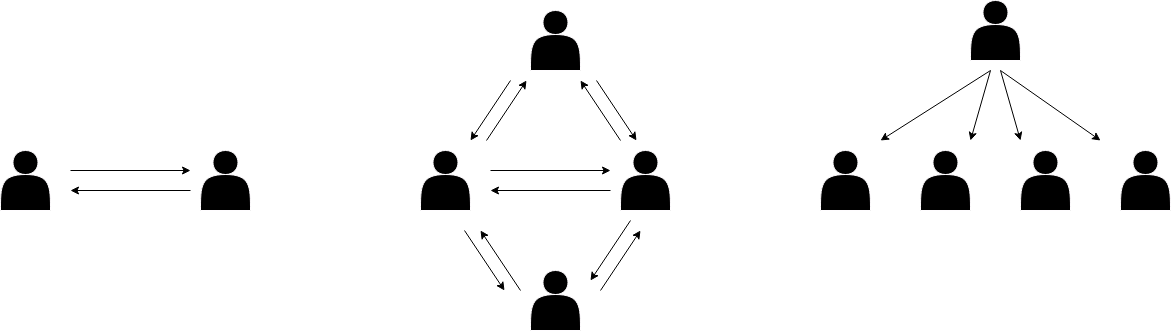
\includegraphics[width=0.7\textwidth]{img/three-types}
\caption{The three types of video conferencing.}
\label{fig:three-types-video-conferencing}
\end{figure}

With video conferencing, people need to send and receive video streams, and we want to do this ideally in real time.
A standard for that is WebRTC, and it is now widely supported in browsers (97.77\% of browser versions used) \cite{
noauthor_webrtc_nodate}. WebRTC is both a protocol and an API that can be used for many things, including video and audio communication.
Matrix even has support for WebRTC and uses it in their client Element \cite{noauthor_element_nodate}. In our
implementation, we will use WebRTC to send video and audio streams. These streams eventually need to arrive at
the other participants in the call, however it can take many different paths to get there depending on the setup of
the network.

The first option is to send the video and audio streams peer-to-peer (P2P). This means that the people in
the call send their stream to every other person in the call. This option does not need a server to manage or
distribute the audio and video stream, ensuring that the hub server has no extra load. The hub server simply
facilitates the call setup. However, with every extra participant, every user needs to send/receive more and more
data. With every new user, every client needs to use more resources and at some point, a bottleneck is
reached, and loss of data will occur. This is a very privacy-friendly method since the server has no access to the
video conferencing data being sent and the users have full autonomy to choose who can receive their video data.
However, due to the limited number of participants, this solution is not feasible.

Another option would be to have a Multipoint Control Unit (MCU). An MCU takes in many media streams, possibly
converts it to another format, and combines these streams into one media stream. This makes it so that it can work
very well with legacy systems, since an MCU can receive various types of media and then output a standardized
output. For example, this would allow a participant to call in from a phone connection while the other participant
is using a desktop application. The MCU has to encode and decode all the incoming media signals, which makes it
costly for the hub at large scale, since this is a computationally intensive task. From a security and privacy
perspective, this solution is not ideal, since the server has access to all the unencrypted video and audio data,
which would mean that the server could potentially listen in or even impersonate someone on the call.

Lastly, we have an architecture with a Selective Forwarding Unit (SFU). An SFU behaves in a way like a switch where it
would selectively forward streams between clients, it does not interact with the video streams so it would work
similarly with encrypted and unencrypted data. From a user perspective, we only need to talk to one server, and we
send and receive all our data through that server. The server simply forwards and thus does not distinguish data
coming from a user or another SFU, which in turn means that we can have multiple SFUs working together to relieve
the load. This can increase the scalability of the system in terms of the number of participants or the quality of the streams when
participants are geographically far apart. An SFU provides a compelling balance of scalability and privacy, which is
why we will use this in our implementation.

\begin{figure}[!hbt]
\centering
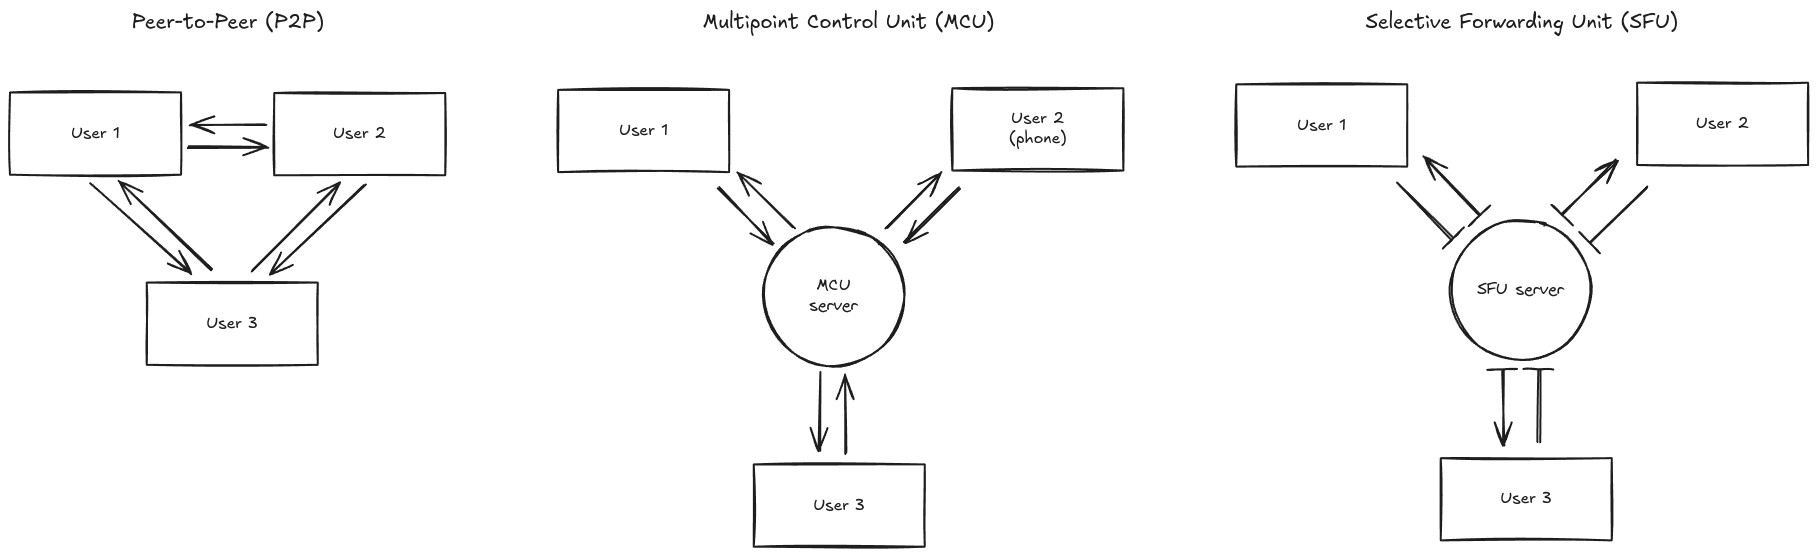
\includegraphics[width=0.7\textwidth]{img/thesisDPD}
\caption{The three options}
\label{fig:three-options-video-conferencing}
\end{figure}

PubHubs for now is only a web based app and we will only focus on the web based video conferencing solutions. This means
that we do not need the legacy support that an MCU provides. We also do not want to have the server have access to the
video and audio data. This leaves us with the SFU and P2P. Since we want to have a scalable solution, we will use the SFU.
Perhaps to save on server bandwidth and to have a more privacy-friendly solution, we can use a P2P network for one-on-one
conferencing. This is something we will look into in future work.

\section{Matrix and Element call}
\label{sec:matrix}
As mentioned previously, PubHubs is built upon Matrix. Matrix is an open-source network for secure, decentralized
communication. It is built on an open standard, which means that anyone can build a client or server that is fully
compatible with the Matrix protocol. User can even make proposals to change the protocol, which can then be voted on
by the community. This protocol is continuously changing depending on the use cases of their users. These changes
are then implemented in the multiple implementations of the protocol. The most well-known implementation is Synapse,
which is the reference implementation of the matrix protocol and is also used by PubHubs.

PubHubs can be considered a layer on top of matrix, which handles the identity management and adds some extra features.
A hub will have to deploy a matrix homeserver, in this case synapse, and their hub client. This also means that you can
access hubs using any matrix client, with the downside that some features are not available in all clients, such as
requesting attributes using Yivi. Matrix is the fundamental layer of PubHubs, and it is important to keep in mind
when designing and implementing new features. When designing the video conferencing solution, we will have to keep
in mind the matrix protocol and only deviate from it when absolutely necessary.

It is important to note that when talking about Matrix, it sometimes refers to the protocol and sometimes to the
reference implementation. In this research, we will mostly talk about the protocol and not the implementation. These
should be the same, but from time to time, there are differences. For instance, when a new feature is in the protocol
but not yet implemented in the reference implementation. We are mostly interested in proposal 3401 \cite{
noauthor_matrix-spec-proposalsproposals3401-group-voipmd_nodate}, since here matrix added functionality for video conferencing. This proposal
can be applied to all the above-mentioned server setups and describes a protocol for video conferencing.

The same team that built matrix is also building Element \cite{noauthor_element_nodate}, which is an open-source matrix client.
A new feature was added to Element called Element call, which serves as an example implementation of proposal
3401 \cite{noauthor_matrix-spec-proposalsproposals3401-group-voipmd_nodate}. They started by using peer-to-peer video conferencing, since this more closely resembled the
decentralized infrastructure of Matrix. However, this turned out to not be the best solution since it allowed for a
maximum of 7 participants and video conferencing required numerous computer  resources from participants. Recently,
they have released a new version that makes use of an open-source SFU called Livekit \cite{noauthor_livekit_nodate}.

We will use this implementation as a guide during our research; however, we will evaluate all the different choices
made for Element call and deviate from them based on the requirements of PubHubs. When using Livekit we can easily
implement features like noise suppression or video simulcast (Sending multiple video streams with different
qualities, to dynamically choose the quality according to a user's internet connection). On the other hand it
also makes PubHubs dependent on Livekit, which is a third-party service.


\chapter{Requirements}
%\section{CIA}
%The CIA triad is a model designed to guide policies for information security within an organization. The model
%consists of three core principles: Confidentiality, Integrity, and Availability. These principles are used to
%evaluate the security of an information system. We will

\section{Confidentiality}
Confidentiality is the principle that information is not made available or disclosed to unauthorized individuals,
entities, or processes. In the context of video conferencing, this means that the video and audio data should only
be available to the participants in the call. Even the server should not have access to the video and audio data. We
can achieve this by having end-to-end encryption. The data is encrypted on the client side and only decrypted by
the receiver on their client side. If the server does not know the encryption keys, then it will not have access to
the video and audio data.

This end-to-end encryption should be fast and secure since the data is sent in real-time. If the encryption and
decryption are computationally expensive, the latency will increase, which will result in a poor user experience. We
also do not want huge system requirements for the clients, since PubHubs should be accessible to everyone.

Some conversations might be sensitive, so we want to make sure that only the users currently in the call can
decrypt the video and audio data. We do not want new users to be able to decrypt the video and audio data from
before they joined the call, this is called forward secrecy. This is a feature that is not strictly necessary for
video conferencing, but this way we can cryptographically ensure that the video and audio data is only available to
the participants that the user can see in the call.

\section{Integrity}
Integrity is the principle that information is protected from unauthorized modification. For video conferencing, transmission integrity
is crucial. Transmission integrity ensures that the streams are received without manipulation during transit.
We can achieve this by having an authenticated encryption scheme, such that we can verify that the data is coming from
the right participant and has not been tampered with.

We also want to make sure that the video and audio data is not modified by the server. This is a bit more difficult
since we need to trust the server to forward the video and audio data to the other participants. If we take the server
to be honest but curious than we need to prevent the server from being able to modify the data. It is therefore crucial
that the server does not have access to the encryption keys, since this would allow the server to decrypt the data and
potentially modify it.

We consider the system integrity to be out of scope for this research. This means that we do not consider the
possibility that the server or the client is compromised. This is a valid threat, but these are the same assumptions
that are made in Pubhubs.

\section{Availability}
Availability is the principle that information is available and accessible when needed by authorized individuals,
entities, or processes. In the context of PubHubs, this means that the video conferencing solution should be able to
handle a large number of participants without compromising the functionality of the rest of PubHubs. We want the
video conferencing solution to be available to all users, but more importantly we do not want a video call to slow
down the rest of PubHubs.

We saw previously that we can have a bottleneck when using P2P video conferencing, since every user needs to send
and receive more and more data with every new participant. This is not a scalable solution, and we will need to use
an SFU. These still have a limit on the number of participants, but this limit is based on the SFU servers resources.

This can be an attack vector, since an attacker can try to overload the hub server by creating many video calls. We
therefore need to have the possibility to have the SFU on a separate server as well as the possibility to scale the SFU
server horizontally. This means that we can deploy multiple SFU servers and have them work together.
This way, the load can be distributed over multiple (separate) servers, and not impact the rest of PubHubs.

\section{Authentication}
Authentication is the principle that the identity of a user can be verified. In the context of video conferencing,
this means that we should be able to verify that the person we are calling is who they say they are. In PubHubs, we
only have a pseudonym, which is a local identity. For some use cases this might be fine, however for some use cases
such as online consultations, we want to be sure that we are actually calling a doctor.

We could require certain attributes to be disclosed before a user can join a call. For example, a hub
can require that a user has a certain age before they can enter a room. These attributes can be the same for both
clients (symmetric) or it can be different attributes (asymmetric). For example, the doctor should disclose their license, but the patient should only
disclose their name. We use Yivi to request and verify these attributes.

We might also want to possibility to verify the attributes of the user in the call ourselves. We also consider this out
of scope for this research, since this is a feature that is not present in PubHubs. For now we trust the server to
verify the identity of the user.

\section{Design}
We want the video conferencing solution to be easy to use and understandable. It should also have some quality of life
features that we come to expect from video conferencing solutions. We want to have basic features like muting the
microphone or the camera, seeing who is in the call, and sharing your screen. We also want to have some more advanced
features like noise suppression and video simulcast. These features are not strictly necessary, but they can greatly
improve the user experience.

PubHubs is a platform that is still in development and is constantly changing. This means that the video
conferencing solution should be able to adapt to these changes. PubHubs is also meant as a very configurable platform
where hubs can enable or disable certain features. This means that the video conferencing solution should be able to
be disabled without affecting the rest of PubHubs.

We can achieve this by having the video conferencing solution completely isolated from the rest of PubHubs.
This means that we will need to have separate data store instead of extending the currently used data store.
Similarly, we will need to have separate endpoints which the video conferencing solution will use,
instead of extending the current endpoints. In general we want to have a clear separation between the video conferencing
solution code and the rest of PubHubs.

\chapter{Proposed solution}
The proposed solution has multiple parts. We will first discuss the server setup, then the video conferencing flow
and lastly the encryption. We will also discuss the front end setup, which is not strictly necessary for the video
conferencing solution, but is included in this prototype. We have included a diagram which shows the different parts
and how they interact with each other.

In the figure, the user is using the PubHubs client to join a room. We can see the PubHubs central server, the hub
server, and the livekit server. The PubHubs central server is used to authenticate the user, the red line shows that
the user is not yet authenticated and the green line shows that the user is authenticated. In the figure we can also see
the contents of the videoCall store, which is used in the hub client. This will be discussed in the following sections.

\begin{figure}[!hbt]
\centering
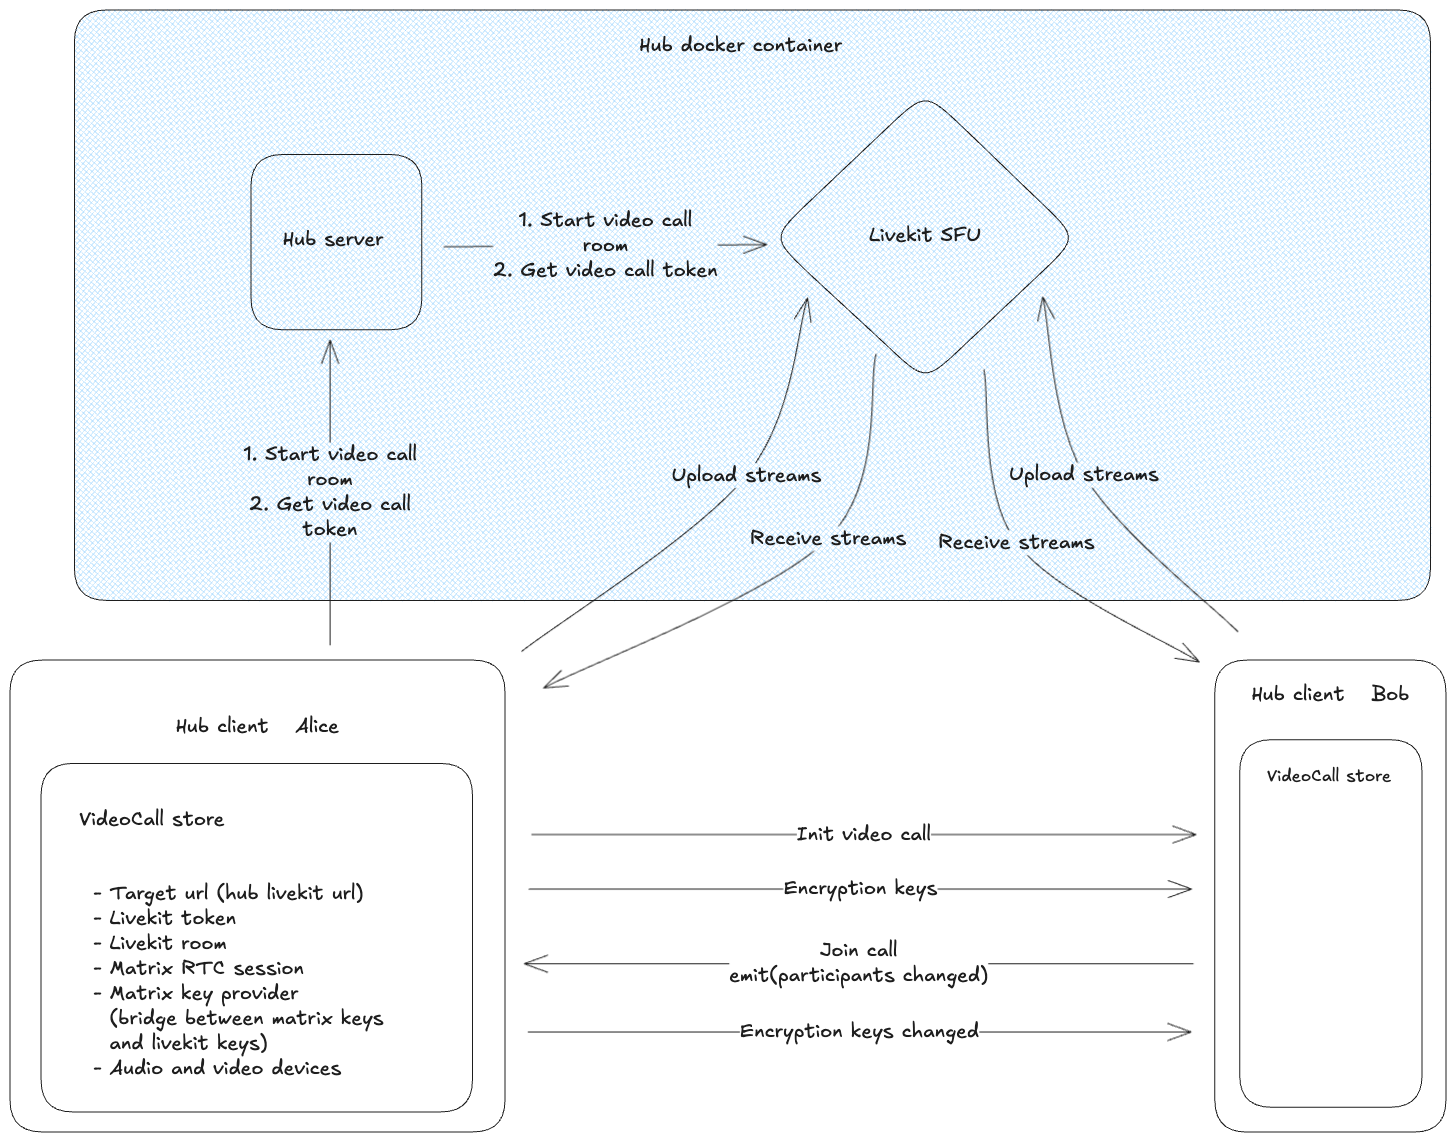
\includegraphics[width=1\textwidth]{img/PH_videocall.excalidraw.png}
\caption{Video conferencing setup}
\label{fig:video-conference-setup}
\end{figure}


\section{Server setup}
The hub server needs some changes to be able to handle video conferencing. Firstly, we will now also need to deploy a
Livekit server instance. This livekit server functions as an SFU and will forward all the video and audio traffic
between the different clients. This server will not see the video conferencing data since they are
encrypted and the server does not have access to the keys. The only thing that the livekit server sees is the local
pseudonym of the user, which the hub server already knows and thus does not leak additional data.

We chose Livekit since it is open-source and can be easily integrated with PubHubs, since the server is written in
Python. Livekit is also used by Element call, which we used as a reference implementation during development. We
also get some additional features like noise suppression and video simulcast, without having to implement them
ourselves. Furthermore, Livekit is simple to configure, can scale very well and can be easily deployed with docker.

Livekit still needs to authenticate the users, it uses a token for this which is seperate from the PubHubs
authentication token. This token is generated by the livekit server but can only be requested by the hub server.
For this we have set up a new endpoint on the hub server such that the user can request a livekit token. The flow is
as follows: The user requests a livekit token from the hub server, the server authenticates the user and checks if
the user is allowed to join the room. If the user is allowed to join the room, the server will request a livekit
token from the livekit server and return this token to the user.

We do the authentication on the hub server in a similar way to the secured rooms. Currently, we only check if
the user is allowed to join the room, however we can also require the user to disclose
certain YIVI attributes. This can easily be changed in the future since we can repurpose the code which is used to
request YIVI attributes for secured rooms. For now, we consider the inclusion of these attributes out of scope since
you can have a similar result by only allowing video conferencing in secured rooms (which have the required
attributes).

The hub server authenticates the user by checking the PubHubs authentication token on the request. These tokens are
the same as when a user requests any other data from the hub server. The response to this call will be an
access token from livekit for this pseudonym and for this room. This token is used when sending and receiving data
from the livekit server, non-authenticated media will be rejected. This token is only valid for the room and the
pseudonym, so the user cannot use this token to join another room or use another pseudonym. Ideally, we would not
have another token besides the PubHubs token since if we would invalidate one of these two tokens we should probably
also invalidate the other. Managing this can and will lead to problems later on. However, having these two tokens
allows us to have a separation between the hub server and the livekit server. This way, we can even host the livekit
server on a physically different server than the hub server, which would be beneficial for the scalability of the
system.

The livekit server can handle a lot of traffic, but when the hub is considerably large and has numerous video calls, it
might be a good idea to have a physically separate livekit server. This way, the hub server will not be overloaded with
video traffic and can still serve the rest of the users. The livekit server can also scale horizontally to handle
more traffic. This is simply a matter of deploying more livekit servers and configuring them to work together.
Livekit provides a CLI tool which can give an indication what the maximum number of users is that a livekit server
can handle. This way, the hub server can decide when to scale up the livekit server.

To give some indication, a livekit server running in a Google cloud compute instance with 16 cores (
c2-standard-16), has around 85 \% CPU utilization when 150 users with 720p video and audio are connected
\cite{noauthor_benchmarking_nodate}. The hub sever can also choose to completely outsource the livekit server.
Livekit provides a paid service where they will host the livekit server for you. This service scales
automatically, and the servers are distributed globally. This way the users will always have a proper low
latency connection to a livekit server. This, however, is a tradeoff between privacy and ease of use. When using
the livekit service, livekit service will not have access to the video conferencing data, but they will have access to
the hub pseudonyms of the users and other metadata (such as duration of the call, ip address of the user, etc). This
is a tradeoff that the hub server will have to make, but we do not recommend to self host the livekit server.

\section{Video conferencing flow}
Our design also includes a video conferencing flow. The video conferencing flow describes the protocol and sequence
of steps that the clients (users) will follow to set up and join a video call.
This is a crucial part of the design, as it directly impacts the privacy and security of the video conferencing solution.
In the video conferencing flow, we deviate somewhat from the original matrix specification. We follow the protocol
when setting up a call, but we do not implement the parts of the protocol which are used to manage the call. For
instance, in the protocol the user shares their media devices and whether their devices are muted. We will not use
this since livekit can handle this for us. We only need to know that a call has started in a room and the encryption
keys of the participants. Livekit will provide us with an endpoint where we can send and receive our data, which in
turn forwards it to the others in our room.

We will thus only use the matrix protocol for setting up the room and sending the keys. This approach is also what
matrix intends to do moving forward, as they have specified in a presentation \cite{nirve_matrixrtc_nodate}. The
matrix team now support both solutions in their client SDK.

\begin{figure}
\centering
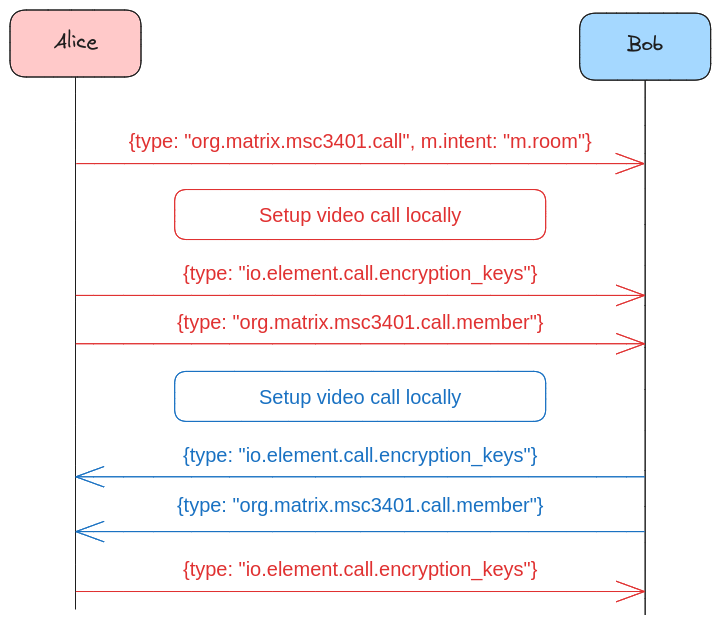
\includegraphics[width=0.6\textwidth]{img/Callflow.excalidraw.png}
\caption{The video conferencing flow}
\label{fig:video-conference-flow}
\end{figure}

To understand the flow, we will go through the flow of Alice starting a call with Bob.
When Alice wants to start a call with Bob, she will send a call event with an intent. This intent can be
everything from having the room automatically join to ringing the other participants. We did not implement
these different behaviors since it was out of scope. After this, Alice's client will set up the video conferencing
screen, this is where she can choose her camera and microphone. When she is ready, Alice will send her encryption
keys and will send to the others that she is a member of the call. She will then wait for any changes to the
participants, if that happens, she will update her keys and send them to the others.

Bob will receive the call event and decides to join the call. His client will set up the video conferencing
screen where he can choose his camera and microphone. When he is ready, Bob will send his encryption keys and will
send to the others that he is a member of the call. Since Alice can see that there is a new participant, she will
update her keys and send them to Bob. Now they have all the keys of all the participants, and they can decrypt their
video and audio streams.

Alice sent her keys twice which is not strictly necessary, however using this we can have a simple code base
without having to check if the keys are already sent. The setup of a call is now the same, regardless whether
the call is new or already ongoing. This makes the code easier to understand and maintain.

\section{Encryption}
For end-to-end encryption, we need to encrypt locally on the clients' device. For that, Livekit provides an e2ee worker,
which encrypts and decrypts incoming messages. This worker is a web worker, which is a separate
thread that runs in the background. This way, the main thread is not blocked by the encryption and decryption
process. The worker uses the Web Crypto API, which is a widely used and tested API for encryption and decryption.
These APIs are now common in all modern browsers, so we can be sure that the encryption and decryption will work on
all devices.

Livekit uses Advanced Encryption Standard cipher in Galois/Counter Mode (AES-GCM)\cite{daemen_rijndael_nodate}\cite{
mcgrew_galoiscounter_nodate}, to encrypt and authenticate the frames. This is a widely used and researched block
cipher. It is also very fast and efficient, even working well on slower devices.

The main problem at hand here is key management. For the encryption to work, we do need the keys from all
participants. To get these keys, we followed the matrix specification for ease of implementation and code
sustainability. As of the writing, matrix is in the middle of transitioning to a new spec where the client can more
directly request, revoke and rotate keys of the participants. Although we believe this would be a better solution, we
decided to stick with the current implementation. This is because the new key management specification is not yet in
the official Matrix specification.

Whenever we are in a call, we subscribe to a \lstinline[language=js]{Matrix\_RTC\_Session}. This session handles
memberships and properties of a session. This will give us messages when a new user is added or when the keys are
updated. Whenever we get an updated key message from the \lstinline[language=js]{rtc\_session}, we pass it through
livekit, which in turn updates the keys and derives new keys from that key. It simply takes the key from \lstinline[
language=js]{matrix\_rtc} and uses that as a seed. Although it is not implemented, users can also rotate their keys.
This is a feature that is supported by livekit, but we did not implement it since it was out of scope. Other complex
key generation schemes are also possible and can very easily be implemented.

We use the implementation of matrix to send the keys, it does so by sending the keys as special messages in a matrix
room. This is not ideal, since the keys are sent in the clear and can be read by the server. However, since the
server does not have access to the video and audio data. This also prohibits us from having forward secrecy since
if you are in the room but not in the video conference, you can still read the keys from before you joined the call.
Matrix has functionality to send these keys via private direct messages to the participants in the call. However, this
feature does not work with their new end-to-end encryption library. We have been in contact with the matrix team, and
they are working on this feature, so we decided to leave the code as is and wait for the new implementation. This
means that until we have the new implementation, we do not have full forward secrecy.

Since we need to initialize the matrix crypto library for the encryption, we can very easily enable end-to-end
encryption for other messages in PubHubs. We have done some experiments with this, which we will discuss in future
work.

\section{The code and frontend}
\begin{figure}[!hbt]
\centering
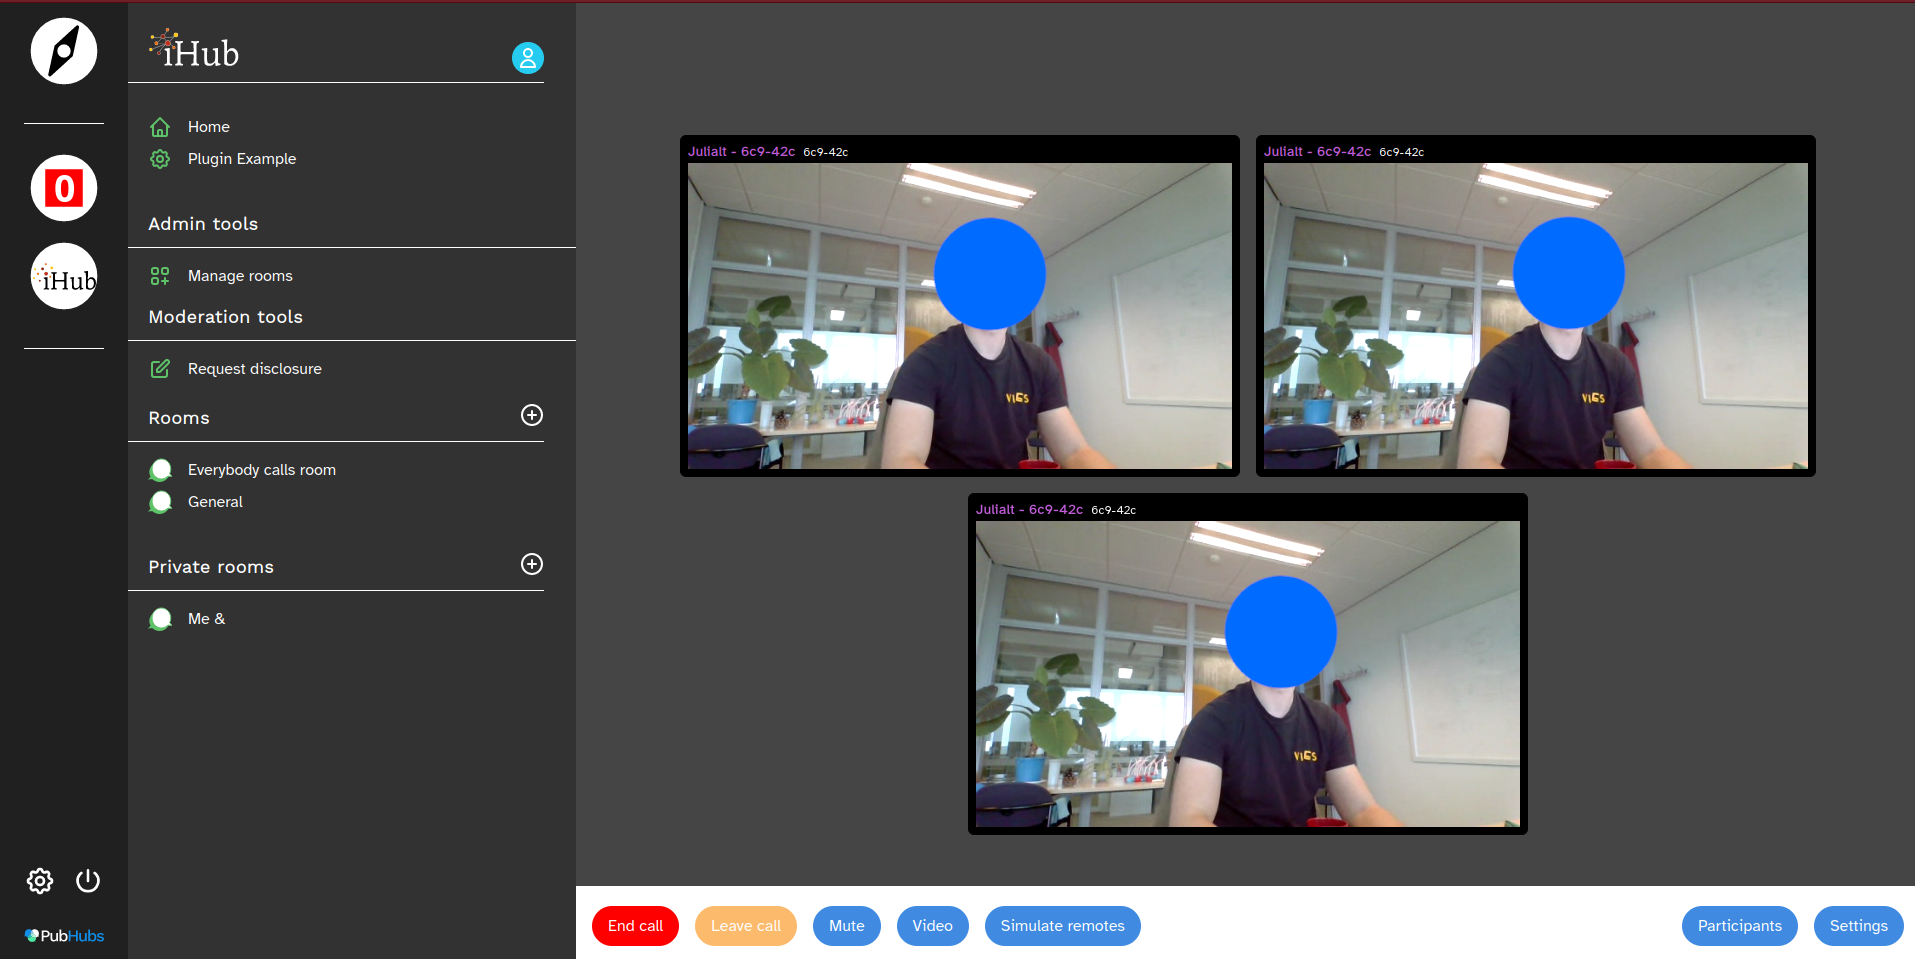
\includegraphics[width=0.8\textwidth]{img/frontend.png}
\caption{The current frontend}
\label{fig:front-end-setup}
\end{figure}

The video conferencing client is developed as an isolated component within PubHubs. This separation allows the
video conferencing solution to be toggled on or off using a feature flag.
This also means that the code is written in a way such that it is isolated from the rest of the PubHubs codebase.
We have a separate store for the video conferencing data, which is only used in the video conferencing code.
This store is used to store the call information, such as the room name, the participants, and the encryption keys.

The video conferencing code is written in the hub client code. We did this so that the video conferencing code is in
line with the rest of pubhubs codebase.
Having the code in the hub client also prevents the need to transmit sensitive data (e.g., room name, LiveKit token,
and SFU URL) to the global client, which could expose hub and room information to the global client unnecessarily.

This also has some other implications, namely that the hub can change the video conferencing solution.
This would enable the hub to adapt the video conferencing solution to their needs, such as requiring certain
attributes to be disclosed before joining a call.
This could also lead to inconsistencies in the video conferencing solution between different hubs, which could be
confusing for the users. This is a tradeoff that was already made in PubHubs, and the other features that run in the
hub client have the same implications.

By having the video conferencing code inside the hub client means that is inside the hub client Iframe.
This turned out to be a problem, when requesting Camera and Microphone access. Because of security reason the
sandbox attribute is set on the Iframe. This means that the Iframe cannot request certain secure attributes.
Access to the camera and microphone are considered secure attributes.
To allow access without removing the iframe’s sandbox attribute, we opted to add the allow attribute and added
permissions for camera and microphone access.
This approach balances security with functionality by enabling device access without relaxing all sandbox restrictions.

Currently, the front end for the video conferencing client is simple and is responsive for up to 5 persons, after which
the video tiles will be cut off.
The primary focus was on back-end implementation, but we still developed a primitive interface which can be easily
extended in the future.
We followed PubHubs’ design principles and reused as many components as possible to ensure that the user interface
remains cohesive with the rest of the platform. The frontend is built to be
reactive, allowing smooth adaptation to changes in participant count or other call settings.
Currently little work in the backend is needed to make the video conferencing client production-ready, but the
frontend still needs some work. This is something that can be done in the future, but is out of scope for this
research.



\chapter{Evaluation}
\section{}

% \newpage
% \section{Research question}
% The main research question will be \textbf{“How can we design and implement an authenticated video conferencing
%     solution within PubHubs that balances privacy, security, and usability?”}. This main question creates several
%     sub-questions. We will divide these up into three different categories.

% \textbf{Privacy}
% For PubHubs privacy is one of their core values and during the creation and development of PubHubs certain
%     decisions have been made regarding privacy. These decision should be considered and can be formulated into
%     these sub-questions:

% — What information or metadata should we allow leaking to achieve authenticated video conferencing, regarding the
%     current PubHubs privacy principles?

% — How can we balance essential call features, like visible call status, with a commitment to user privacy?

% \textbf{Encryption}
% One of the foremost considerations in GDPR compliance for video conferencing is the implementation of end-to-end
%     data encryption. This requires an encryption scheme which is user-friendly, has low computational overhead, and
%     still has appropriate security.

% — What encryption scheme is best suited for authenticated video conferencing in PubHubs, weighing user experience
%     and computational overhead while ensuring optimal security?

% \textbf{Development}
% While doing the research and writing the code for it, we should also keep in mind the current development setup for
%     PubHubs. This means that we should keep in mind which technologies they are using now and remain in those
%     ecosystems. This makes it so that the code can be more easily maintained in the future. PubHubs allows hubs to
%     create their own version of the hub client, which should be considered when creating the video conferencing
%     client.

% — How can we develop a video conferencing prototype within the existing PubHubs ecosystem, while simultaneously
%     considering different hub client implementations?


\chapter{Future work}
\section{Speaker-to-audience}
As mentioned previously, we have three types of video conferencing. We have only implemented the one-on-one type and
the group type. However there might still be a need for speaker-to-audience type of video conferencing, for instance
when a hub is owned by a municipality and they want to give a speech. This type of video conferencing has different
requirements and the current video conferencing setup would be inefficient.

We have a speaker who sends their video and audio stream to all the audience members. The audience members only send
their video and audio stream to the speaker. The later we is not even needed at all or for all members. This is not
achievable with the current setup, since we would need to send the video and audio stream to all the audience members.
Currently it would be hard to develop this feature without a clear use case, since depending on the use case we can
see what we can optimize. More research and requirements engineering is needed to build such a feature.

% speaker-to-audience
\section{Video conferncing access management}
When a user wants to join a call, this solution only checks if the user is a member of the room. This can be a
redular room, direct message room (1-to-1 room) or even a secured room. With the later we know that the user has
disclosed the required attributes to join the secured room. However, for some use cases we might want to have more
control over who can join the call. For instance when we do not want to allow all users to join a call. In direct
messages rooms we might want to have the user disclose their identity before they can join the call, to
make sure we are actually calling the right person and not an impersonator.

If we were to implement this, we would need to know what the exact use cases are and what the requirements are for
these use cases. Currently we can simply use the secured rooms to create a similar effect, however this might not be
a very elegant solution for some use cases. Currently more research is needed to determine what the exact requirements
are for this feature.

\section{End-to-end encryption for other messages}
The current implementation only encrypts the video and audio data. In order to enable this, we need to initialize the
matrix crypto library. This library can also be used to encrypt the other messages in Pubhubs. We have experimented
with this and have found that it is very easy to enable this. However, some Pubhubs features did not work as expected
when we enabled this. This is something that is relatively easy to overcome, but more research is needed to determine
what the other implications are of enabling this feature.

There are also some considerations which need to made before this feature is production ready.
For instance, how would end-to-end encryption work with multiple devices? Currently, the encryption keys are stored in
the local storage of the browser. This means that when you switch devices, you will not have the encryption keys and
thus cannot decrypt the messages. Currently, Pubhubs focusses on the web client, but in the future they might want to
have a mobile client be on par with the web client.

Another consideration is how to handle moderation. One of the main features of Pubhubs is privacy friendly moderation.
However, when the messages are end-to-end encrypted, then the moderator needs to have access to the encryption keys to
moderate the messages. There are other multiple considerations which need to be made depending on the specific
moderation used in Pubhubs \cite{noauthor_group_nodate}.

\newpage
\bibliographystyle{acm}
\bibliography{references.bib}

\end{document}